\documentclass[border=10pt]{standalone}

\usepackage{tikz}
\usepackage{tikzsymbols}
\usetikzlibrary{calc,patterns,shapes.geometric}

\def\centerarc[#1](#2)(#3:#4:#5){\draw[#1] ($(#2)+({#5*cos(#3)},{#5*sin(#3)})$) arc (#3:#4:#5);}

\begin{document}
	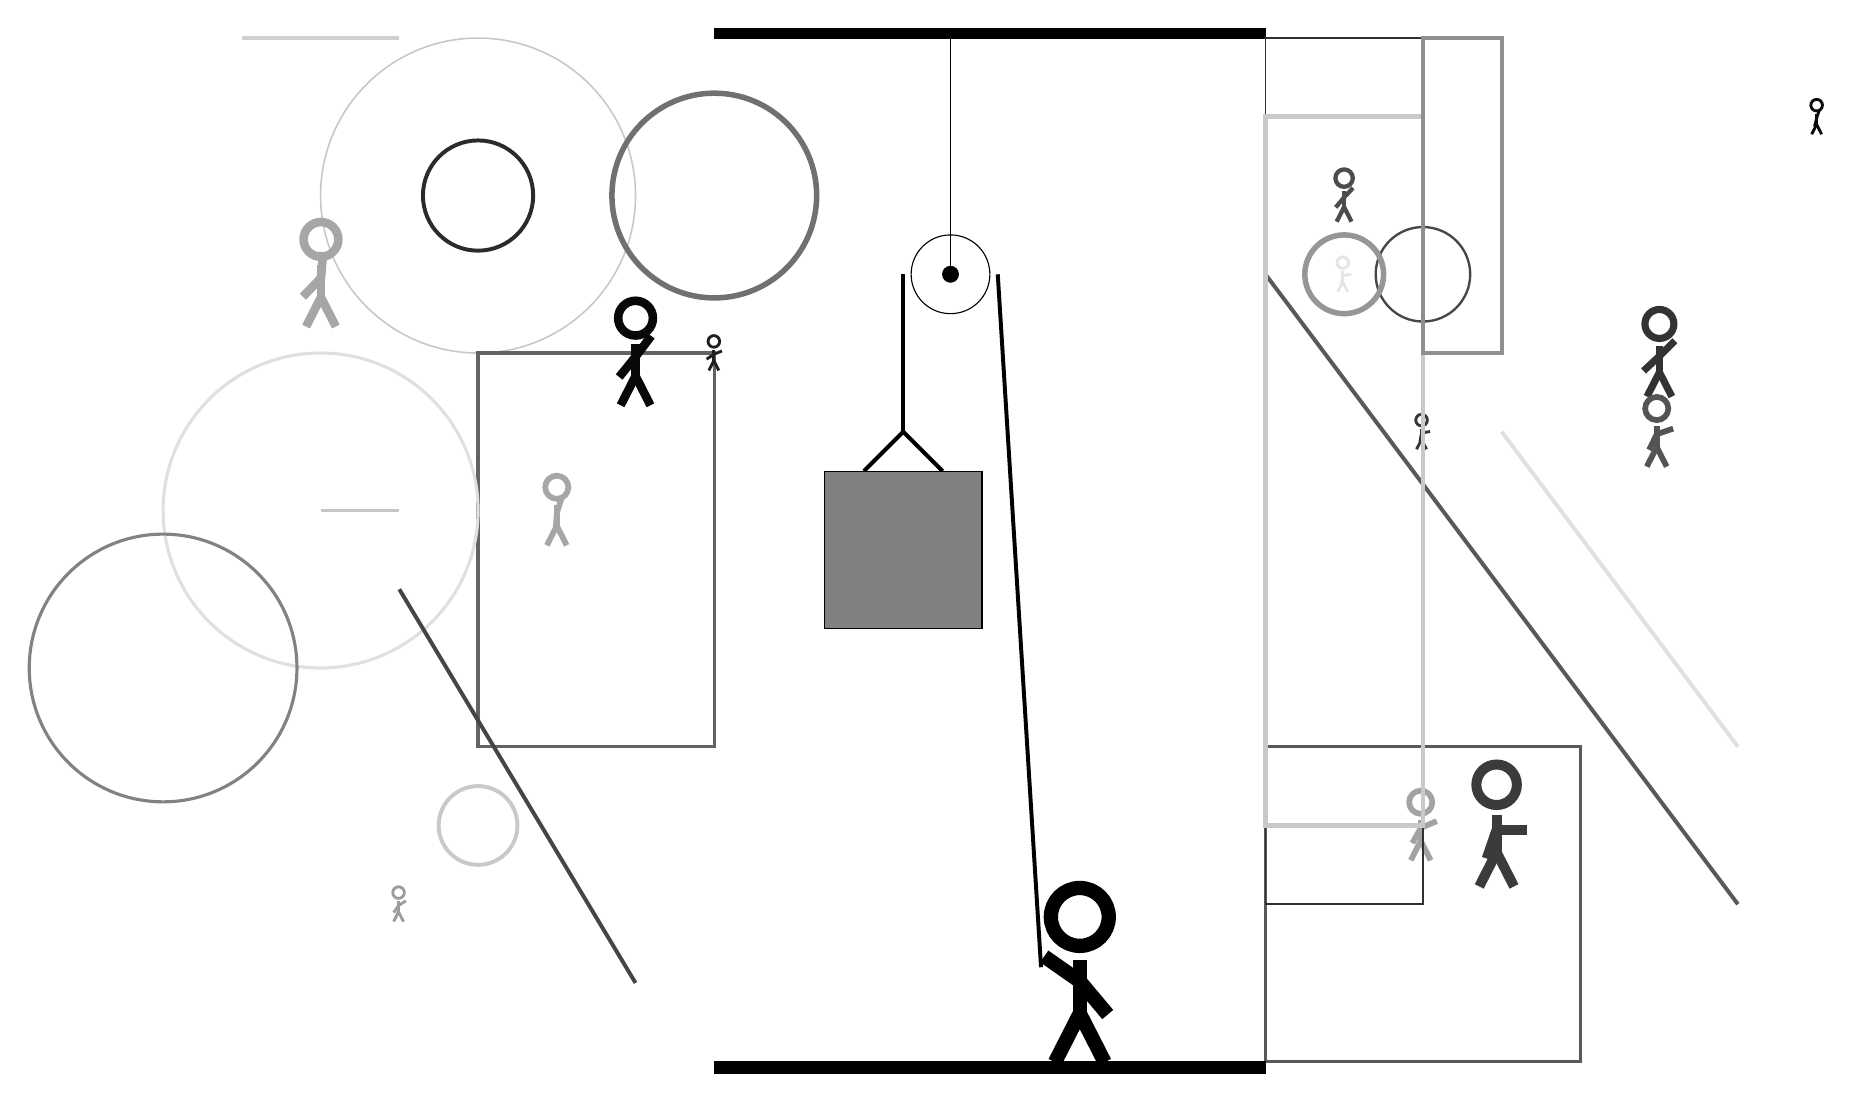
\begin{tikzpicture}
		%%%%% START %%%%%
		
		\draw[fill=black] (-2, 10) rectangle (5, 10.125);
		
		\draw (1, 7) circle (0.5);
		\draw[fill=black] (1, 7) circle (0.1);
		\draw (1, 10) -- (1, 7);
		
		\draw[line width=0.5mm] (-0.1, 4.5) -- (0.4, 5.0) -- (0.9, 4.5);
		\draw[fill=black!50] (-0.6, 4.5) rectangle (1.4, 2.5);
		
		\draw[line width=0.4mm, color=black!65] (5, 1) rectangle (9, -3);
		
		\draw [line width=0.2mm, color=black!22](-5, 8) circle (2.0);
		\draw[line width=0.4mm, color=black!61] (-2, 1) rectangle (-5, 6);
		\node[line width=0.5mm, color=black!35] at (-4, 4) {\Strichmaxerl[4][86][72]};
		\draw[line width=0.4mm, color=black!26] (7, 3) rectangle (7, 3);
		
		\node[line width=0.3mm, color=black!96] at (12, 9) {\Strichmaxerl[2][76][71]};
		
		\node[line width=0.5mm, color=black!80] at (10, 6) {\Strichmaxerl[5][43][45]};
		\draw[line width=0.5mm, color=black!65](5, 7) -- (11, -1);
		\draw [line width=0.4mm, color=black!12](-7, 4) circle (2.0);
		\draw[line width=0.5mm, color=black!19](-6, 10) -- (-8, 10);
		
		\draw[line width=0.5mm, color=black!12](8, 5) -- (11, 1);
		\draw [line width=0.3mm, color=black!72](7, 7) circle (0.6);
		\draw[line width=0.5mm, color=black!73](-3, -2) -- (-6, 3);
		\node[line width=0.3mm, color=black!97] at (-3, 6) {\Strichmaxerl[6][51][53]};
		\node[line width=0.7mm, color=black!39] at (-6, -1) {\Strichmaxerl[2][56][32]};
		\node[line width=0.5mm, color=black!77] at (8, 0) {\Strichmaxerl[7][71][0]};
		\draw [line width=0.4mm, color=black!49](-9, 2) circle (1.7);
		\node[line width=0.2mm, color=black!79] at (7, 5) {\Strichmaxerl[2][79][10]};
		\node[line width=0.2mm, color=black!67] at (10, 5) {\Strichmaxerl[4][64][19]};
		\node[line width=0.4mm, color=black!36] at (7, 0) {\Strichmaxerl[4][61][23]};
		\draw[line width=0.2mm, color=black!81] (5, -1) rectangle (7, 10);
		
		\draw[line width=0.6mm, color=black!21] (7, 9) rectangle (5, 0);
		\node[line width=0.4mm, color=black!70] at (6, 8) {\Strichmaxerl[3][50][47]};
		\node[line width=0.4mm, color=black!10] at (6, 7) {\Strichmaxerl[2][82][8]};
		\draw [line width=0.5mm, color=black!83](-5, 8) circle (0.7);
		\draw[line width=0.5mm, color=black!44] (7, 6) rectangle (8, 10);
		\draw [line width=0.7mm, color=black!41](6, 7) circle (0.5);
		\node[line width=0.2mm, color=black!88] at (-2, 6) {\Strichmaxerl[2][34][22]};
		\draw[line width=0.5mm, color=black!22](-6, 4) -- (-7, 4);
		
		\node[line width=0.5mm, color=black!35] at (-7, 7) {\Strichmaxerl[6][46][85]};
		\draw [line width=0.7mm, color=black!56](-2, 8) circle (1.3);
		
		\draw [line width=0.5mm, color=black!21](-5, 0) circle (0.5);
		
		\draw[line width=0.5mm] (0.4, 7) -- (0.4, 5.0);
		\centerarc[line width=0.5mm](1, 7)(0:180:0.6);
		\draw[line width=0.5mm](1.6, 7) -- (2.15, -1.8);
		
		\node at (2.6, -1.9) {\Strichmaxerl[10][-35][-50]};
		
		\draw[fill=black] (-2, -3) rectangle (5, -3.15);
		
		%%%%% END %%%%%
	\end{tikzpicture}
\end{document}